% !TeX document-id = {49b9cd48-9a28-43d8-a1fd-030bc1e37b2e}
% % Konfiguration für Texstudio (Version > 2.9)
% !TeX program = pdflatex
%% !TeX TXS-program:compile = txs:///pdflatex/[--shell-escape]
% !BIB program = biber
% !TeX spellcheck = de_DE
% !TeX encoding = utf8
% !TeX root = Thesis.tex


\newcommand{\authorname}{Manfred Mustermann} 

% Header

\documentclass[
	a4paper,
	%oneside,
	twoside,
	12pt,
	numbers=noenddot,
	openright,	% Kapitel beginnt auf rechter Seite
	titlepage,	% Titelblatt auf eigener Seite
	bibliography=totoc,		% Literaturverzeichnis
	listof=totoc,	% Listen ins Inhaltsverzeichnis
	twoside,  % zweiseitig
]{scrbook}



\usepackage[english,ngerman,shorthands=off]{babel} % Deutsche Sprachanpassungen
\usepackage[T1]{fontenc}    % Silbentrennung bei Sonderzeichen
\usepackage[utf8]{inputenc} % Direkte Angabe von Umlauten im Dokument.
\usepackage{lmodern}					% Umlaute markierbar in PDF
\usepackage{textcomp}       % Zusätzliche Symbolzeichen
\usepackage{microtype}       % Optimierter Rand
\usepackage{amsmath}					% Formeln
\usepackage{graphicx}					% Graphiken einbinden
\usepackage{float}
\usepackage[german]{nomencl}
\usepackage[countmax]{subfloat}
\usepackage{wallpaper}

%\clubpenalty = 10000 % schliesst Schusterjungen aus
%\widowpenalty = 10000 % schliesst Hurenkinder aus


%eigene Packete
\usepackage{makeidx}
\makeindex
%eigene Packete ende

% Farben definieren für package listings 
\usepackage{color}
\definecolor{middlegray}{rgb}{0.5,0.5,0.5}
 \definecolor{lightgray}{rgb}{0.8,0.8,0.8}
 \definecolor{orange}{rgb}{0.8,0.3,0.3}
 \definecolor{yac}{rgb}{0.6,0.6,0.1}
 \definecolor{commentgreen}{rgb}{0.25,0.5,0.37}
 \definecolor{keyred}{RGB}{127,0,85}
 
% C-Quellcode einfügen
\usepackage{listings}
\lstset{
   basicstyle=\scriptsize\ttfamily,
   keywordstyle=\bfseries\ttfamily\color{keyred},
   stringstyle=\color{blue}\ttfamily,
   commentstyle=\color{commentgreen}\ttfamily,
   emph={square}, 
   emphstyle=\color{blue}\texttt,
   emph={[2]root,base},
   emphstyle={[2]\color{yac}\texttt},
   showstringspaces=false,
   flexiblecolumns=false,
   tabsize=2,
   numbers=left,
   numberstyle=\tiny,
   numberblanklines=false,
   stepnumber=1,
   numbersep=10pt,
   xleftmargin=15pt,
  breaklines=true,
  breakatwhitespace=false,
 }
 %selbst eingefügt
 \renewcommand{\lstlistingname}{Quellcode}% Listing -> Algorithm
 \renewcommand{\lstlistlistingname}{Quellcodeverzeichnis}% List of Listings -> List of Algorithms


\setcounter{tocdepth}{3} %Gibt an, bis in welche Tiefe das Inhaltsverzeichnis geht
\setcounter{secnumdepth}{3}

\addto\captionsngerman{
\renewcommand{\figurename}{Abb.}
\renewcommand{\tablename}{Tab.}
} %Sorgt dafürm, dass statt Abbildung Abb. steht und statt Tabelle Tab.
 
\usepackage{titlesec}
\titleformat{\chapter}[display]
 {\bfseries\huge}
  {\filleft\Large\chaptertitlename~\thechapter}
  {3ex}
  {\titlerule\vspace{1.5ex}\filright}
  [\vspace{1ex}\titlerule]

\usepackage{acronym}
\usepackage{glossaries}
\usepackage{wrapfig}
\usepackage{units}
\usepackage{icomma} %Korrekte Abstände bei Dezimalkommas im Mathemodus

% % % %LITERATURVERWALTUNG
	% % % ACHTUNG: Zum kompilieren muss biber, nicht bibtex verwendet werden!
	\usepackage[
		backend=biber,
		style=ieee,
		backref=true,%Referenzen im LieVerzeichnis auf verwendete Seiten im dokument
		isbn=false,
		doi=false,
		eprint=false,
		url=false,
		safeinputenc,
		defernumbers=false]{biblatex} %------------------------------------------------------------------------->war urspünglich true und habe ich auf false geändert (fand ich schöner)
	\usepackage{csquotes}
	
	%\ExecuteBibliographyOptions{sorting=ydmdnt}%Sortierung, none bedeutet nach Vorkommen
	\ExecuteBibliographyOptions{firstinits=true} %Vor- und Mittelnamen als Initialen ausgeben
	\ExecuteBibliographyOptions{maxbibnames=6} %max angezeigte namen, dann auf minnames reduziert und u.a. ergänzt
	\ExecuteBibliographyOptions{minbibnames=4} %siehe maxnames
	\ExecuteBibliographyOptions{maxcitenames=3} %analog für citeauthor, o.ä.
	\ExecuteBibliographyOptions{mincitenames=1} %siehe maxnames

% %Tikz für schöne Zeichnungen:
	% Tikz pakete & optionen
	\usepackage{tikz}
	\usepackage[european,americaninductors]{circuitikz}
	\usetikzlibrary{patterns}
	% % Externalize settings
	\usetikzlibrary{external} 
	\tikzset{external/up to date check=simple}
	%\tikzsetexternalprefix{} %path to graphics ACHTUNG: In header.tex definiert!
	\tikzexternalize%[shell escape=-enable-write18] %option nötig für miktex
	\pgfkeys{/pgf/images/include external/.code={\href{file:#1}{\pgfimage{#1}}}} %Links in pdf zu externen PDF-Bildern für Debug

	% pgfplot pakete & Optionen
	\usepackage{pgfplots}
	
	\usepgfplotslibrary{groupplots}
	
	\pgfplotsset{compat=1.10}
	\pgfplotsset{every tick label/.style={font={\scriptsize\sansmath\boldmath}}}
	\pgfplotsset{every axis label/.style={font={\boldmath\small\sffamily\bfseries}}}
	\pgfplotsset{every legend /.style={font={\boldmath\small\sffamily\bfseries}}}
	\pgfplotsset{every label/.style={font={\boldmath\small\sffamily\bfseries}}}
	
	\pgfplotsset{width=\textwidth}
	\pgfplotsset{grid=both}
	\pgfplotsset{major tick style={thin,black}}% modifies the style ‘every tick’
	\pgfplotsset{minor tick style={very thin,black}}% modifies the style ‘every tick’
	\pgfplotsset{major grid style={thin}} %modifies the style ‘every major grid’
	\pgfplotsset{minor grid style={very thin}} % modifies the style ‘every minor tick’
	\pgfplotsset{minor x tick num=1} %n minor ticks zwischen major ticks(major tiks müssen selben abstand haben)
	\pgfplotsset{minor y tick num=1} %n minor ticks zwischen major ticks(major tiks müssen selben abstand haben)
	\pgfplotsset{xlabel near ticks,ylabel near ticks}
	%For ylabel offsets:
	
	%For ylabel offsets:
	\pgfplotsset{ylabsh/.style={every axis y label/.style={at={(0,0.5)}, xshift=#1, rotate=90}}}
	\pgfplotsset{xlabsh/.style={every axis x label/.style={at={(0.5,0)}, yshift=#1}}}
	%Erweiterung Each nth point mehr als 100 Punkte auslassen
	\makeatletter
	\pgfplotsset{
	/pgfplots/each nth point**/.style={%
	/pgfplots/x filter/.append code={%
	        \ifnum\coordindex=0
	                \def\c@pgfplots@eachnthpoint@xfilter{0}%
	                \edef\c@pgfplots@eachnthpoint@xfilter@cmp{#1}%
	        \else
	                \pgfplotsutil@advancestringcounter\c@pgfplots@eachnthpoint@xfilter
	                \ifx\c@pgfplots@eachnthpoint@xfilter@cmp\c@pgfplots@eachnthpoint@xfilter
	                        \def\c@pgfplots@eachnthpoint@xfilter{0}%
	                \else
	                        \let\pgfmathresult\pgfutil@empty
	                \fi
	        \fi
	}%
	},
	}
	\makeatother
	
	%cycle list für plots, !!!! \addplot+ verwenden!
	\pgfplotsset{
	    cycle list={
	        blue,
	        red,
	        {black, thick, dashed},
	        violet
	    }
	}
	
	



%%%% Abkürzungsverzeichnis %%%%
	%\usepackage[intoc]{nomencl}						% Abkürzungsverzeichnis
	%\usepackage{nomencl}						% Abkürzungsverzeichnis
	%\renewcommand{\nomname}{Abkürzungsverzeichnis}	% Deutsche Überschrift
	%\setlength{\nomlabelwidth}{.25\hsize}			% Punkte zw. Abkürzung und Erklärung
	%\renewcommand{\nomlabel}[1]{#1 \dotfill}
	%\setlength{\nomitemsep}{-\parsep}				% Zeilenabstände verkleinern
	%\makenomenclature
	%eigene version des AK Verzeichnisses
	\usepackage[]{acronym}
	\usepackage{geometry}
	\geometry{a4paper, top=30mm, left=26mm, right=26mm, bottom=35mm,
	headsep=10mm, footskip=12mm} %Legt Seitenränder fest





%%%% Kopf- und Fußzeilen %%%%
	%\usepackage[automark, headsepline, footsepline]{scrpage2}
	\usepackage[automark, headsepline]{scrpage2}		% Kopf- und Fußzeilen
	\pagestyle{scrheadings}
	\clearscrheadfoot
	\ohead{\headmark}
	\ihead{Bachelorarbeit}
	\cfoot{Stand: \today }
	%\cfoot[\pagemark]{\pagemark}
	%\ohead[\headmark]{\headmark}
	%\ihead[Masterarbeit]{Masterarbeit}
	\ofoot{\pagemark}
	\ofoot[\pagemark]{\pagemark}
	%\ifoot{Lehrstuhl für Technische Elektronik}
	%\ifoot[Lehrstuhl für Technische Elektronik]{Lehrstuhl für Technische Elektronik}


% Hyperref als letztes laden
	\usepackage[pdftex,hidelinks]{hyperref} %Für Links im PDF
	\hypersetup{
	  pdftitle    = {Abschlussarbeit Christof Pfannenmüller},
	  pdfsubject  = {Thesis},
	  pdfauthor   = {\authorname},
	  pdfkeywords = {Bachelorarbeit, Pfannenmüller,Basisstation,TDA,XMC4500,Feldstärke,Ortung} ,
	}
%pfade definieren
	\graphicspath{{abbildungen/}}
	\tikzsetexternalprefix{abbildungen/tikz-ext-out/\thesubsection-} %path to graphics
%\tikzset{external/force remake} %uncomment to remake ALL tikz figures
\bibliography{bibliography.bib}
\begin{document}
	\pagenumbering{roman}           

	\begin{titlepage}
\ThisLRCornerWallPaper{0.66}{Abbildungen/Logo/Friedrich_logo_dunkel}
%\begin{center}
%
\includegraphics[width=0.6\textwidth]{Abbildungen/Logo/FAUlogo.eps}
%\end{center}
\begin{figure}

\includegraphics[width=0.45\textwidth]{Abbildungen/Logo/FAUlogo}\hfill
\includegraphics[width=0.27\textwidth]{Abbildungen/Logo/LTElogo}
\end{figure}
%\newline
%\newline
\hspace{0.1cm}	
\center
\LARGE
	\textbf{Lehrstuhl für Technische Elektronik} \\
	Prof.~Dr.-Ing.~Dr.-Ing.~habil.~Robert~Weigel	\\
	Prof.~Dr.-Ing.~Georg~Fischer\\
\vspace{1cm}	

\LARGE
	\textbf{Bachelorarbeit}
\vspace{0.9cm}

\large
im Studiengang\\ \enquote{Elektrotechnik, Elektronik und Informationstechnik (EEI)}\\
\vspace{0.5cm}
von
\vspace{0.5cm}

\LARGE{
\authorname}
\vspace{0.7cm}

\large
zum Thema
\vspace{0.9cm}

\LARGE
\textbf{Aufbau und Inbetriebnahme einer mobilen Basisstation für 
feldstärkebasierte Lokalisierung}
\vspace{1.7cm}

\large
\begin{tabular}{ll}
Betreuer: & Dipl.-Ing. Felix Pflaum \\
 &\\
Beginn: & 25.04.2016\\
Abgabe: & 26.09.2016\\
\end{tabular}
\end{titlepage}

	
	\noindent %die ersten Zeilen eines Absatzes werden nicht eingerückt
	
	% Erklärung

\chapter*{Erklärung}
\label{sec:Erklärung}
%\newpage
%\thispagestyle{empty}
%\noindent
Ich versichere, dass ich die Arbeit ohne fremde Hilfe und ohne Benutzung anderer als der angegebenen Quellen angefertigt habe und dass die Arbeit in gleicher oder ähnlicher Form noch keiner anderen Prüfungsbehörde vorgelegen hat und von dieser als Teil einer Prüfungsleistung angenommen wurde. \\
\\
Alle Ausführungen, die wörtlich oder sinngemäß übernommen wurden, sind als solche gekennzeichnet. \\
\vspace{1.0cm}
\\
Erlangen, den 30. September 2013
\vspace{2.5cm}
\\
Mein Name



	% Kurzfassung

\chapter*{Kurzfassung}
\label{sec:kurzfassung}
\pagestyle{scrheadings}

Ziel der vorliegenden Arbeit war der Aufbau einer Basisstation mit sechs unabhängigen Transceivern. Der Einsatz dieses Aufbaus sollte der späteren Lokalisierung von Sensoren oder anderen Sendern im Sub-GHz-Frequenzbereich um 868 MHz dienen. Die relative Ortsbestimmung zur Basis sollte energieeffizient sein und gleichzeitig eine hohe Auflösung bieten. 
Dazu sollte die genaue Position des Senders auf Basis der unterschiedlichen Feldstärken an den Transceivern eruiert werden. Ausgenutzt werden sollte dabei, das typische integrierte Transceiver die Empfangsfeldstärke selbst auswerten und diese ausgelesen werden kann. Das Erkennen von Übertragungen und das anschließende Auslesen der anfallenden Daten sollte dabei ein Mikrocontroller übernehmen. Zur weiteren Verarbeitung der Daten sollten diese anschließend einem Computer zur Verfügung gestellt werden. Dazu wurde sowohl eine USB- als auch eine Netzwerk-Schnittstelle vorgesehen. Die beim Aufbau der Platine verwendete Hardware basierte zum Großteil auf Bauteilen des Herstellers Infineon. 
Beim Layout der Platine wurden die sechs Transceiver sternförmig und regelmäßig um den Mikrocontroller und dessen Peripherie angeordnet um ein gleichmäßiges Empfangsverhalten aus allen Raumrichtungen zu gewähren. Die Funksegmente der Platine wurden so gestaltet, das diese bei Bedarf abgetrennt und mit einer Kabelverbindung weiter voneinander entfernt werden konnten. Antennen zum Senden sollten über Steckverbinder an die Basis angeschlossen werden.
Der anschließende Softwareentwurf für die Basisstation nutzte zu einem Großteil bereits bestehende Bibliothek und sollte ankommende Übertragungen erkennen, die zur Ortung notwendigen gemessenen Werte abfragen und an den Hostcomputer weiterleiten. 



	% Abstract
\newpage
\chapter*{Abstract}
\label{sec:abstract}
\pagestyle{scrheadings}

Lorem ipsum dolor sit amet, consetetur sadipscing elitr, sed diam nonumy eirmod tempor invidunt ut labore et dolore magna aliquyam erat, sed diam voluptua. At vero eos et accusam et justo duo dolores et ea rebum. Stet clita kasd gubergren, no sea takimata sanctus est Lorem ipsum dolor sit amet. Lorem ipsum dolor sit amet, consetetur sadipscing elitr, sed diam nonumy eirmod tempor invidunt ut labore et dolore magna aliquyam erat, sed diam voluptua. At vero eos et accusam et justo duo dolores et ea rebum. Stet clita kasd gubergren, no sea takimata sanctus est Lorem ipsum dolor sit amet. Lorem ipsum dolor sit amet, consetetur sadipscing elitr, sed diam nonumy eirmod tempor invidunt ut labore et dolore magna aliquyam erat, sed diam voluptua. At vero eos et accusam et justo duo dolores et ea rebum. Stet clita kasd gubergren, no sea takimata sanctus est Lorem ipsum dolor sit amet.   

Duis autem vel eum iriure dolor in hendrerit in vulputate velit esse molestie consequat, vel illum dolore eu feugiat nulla facilisis at vero eros et accumsan et iusto odio dignissim qui blandit praesent luptatum zzril delenit augue duis dolore te feugait nulla facilisi. Lorem ipsum dolor sit amet,
Testos Test von Umlauten wie Ü oder Ö oder anderem.

	%%Abkürzungsverzeichnis
\newpage
\chapter*{Abkürzungsverzeichnis}
\label{sec:ak}
\pagestyle{scrheadings}


\begin{acronym}[CMSIS] %statt Bash die Längste Abkürzung einfügen
	\acro{PCB}{Printed Circuit Board}
	\acro{EDA}{Electronic Design Automation}
	\acro{CAD}{Computer-aided design}
	\acro{SMD}{Surface-mounted device}
	\acro{SPI}{Serial Peripheral Interface}
	\acro{DRC}{Design-Rule-Check}
	\acro{FIFO}{First In – First Out}
	\acro{NCS}{Non-Chip-Select}
	\acro{IC}{Integrierter Schaltkreis}
	\acro{SMA}{Sub-Miniature-A}
	\acro{LQFP}{Low Profile Quad Flat Package}
	\acro{BGA}{Ball Grid Array}
	\acro{JTAG}{Joint Test Action Group}
	\acro{TVS}{Transient Voltage Suppressor}
	\acro{LDO}{Low Drop-Out}
	\acro{SOT}{Small Outline Transistor}
	\acro{STEP}{Standard for the Exchange of Product Model Data}
	\acro{NC}{Numerical Control}
	\acro{IDE}{integrated development environment}
	\acro{GUI}{Graphical User Interface}
	\acro{SDK}{Software development kit}
	\acro{CPU}{Central Processing Unit}
	\acro{USIC}{Universal Serial Interface Channel}
	\acro{ETH}{Ethernet MAC \acroextra{(Ethernet Medium Access Control)}}
	\acro{USB}{Universal Serial Bus}
	\acro{GPIO}{General Purpose Input/Output}
	\acro{ISR}{Interrupt Service Routine}
	\acro{ERU}{Event Request Unit}
	\acro{ERS}{Event Request Select}
	\acro{ETL}{Event Trigger Logic}
	\acro{OGU}{Output Gating Unit}
	\acro{NVIC}{Nested Vectored Interrupt Controller}
	\acro{GND}{Masse \acroextra{(Ground)}}
	\acro{CMSIS}{Cortex Microcontroller Software Interface Standard}
	\acro{MISO}{Master-In Slave-Out}
	\acro{MOSI}{Master-Out Slave-In}
	\acro{ASCII}{American Standard Code for Information Interchange}
	\acro{IRQ}{Interrupt Request}
	\acro{PLL}{Phasenregelschleife \acroextra{(phase-locked loop)}}
	\acro{AGC}{automatic gain control}
	\acro{RSSI}{Received Signal Strength Indication}
	
	
	
	
	%todo: ordnen nach auftrten
%	miso Mosi hinzufügen; GND??
\end{acronym}			% Abkuerzungsverzeichniss


	\tableofcontents
	\thispagestyle{empty}	%Inhaltsverzeichnis auf 2. Seite ohne Seitenzahl
	          
	\pagenumbering{arabic} 
	% Motivation

\chapter{Einleitung}\label{Einleitung}
Hier gehört die Einleitung/Motivation hin. Auf Kapitel \ref{Einleitung} kann so verwiesen werden.

\section{Nötige Programme}
Für die Arbeit mit Latex benötig man eine Tex-Distribution, verbreitet sind hier Miktex und TExlive, empfohlen wird Texlive(\url{https://www.tug.org/texlive/}) in der aktuellsten Version(Upgraden!).

Außerdem benötig man einen Editor, verbreitet sind hier Texniccenter, Texmaker, TexmakerX und Texstudio. Empfohlen wird Texstudio(\url{http://www.texstudio.org/}).

Für die Literaturverwaltung (Erstellen der Bibfiles )kann ein einfacher Texteditor(Notepad++) Texstudio oder (für poweruser) jabref  verwendet werden.


\section{Einige tex Kommandos}\label{sec:texkommandos}
\markboth{Einige tex Kommands}{Einige tex Kommands} %für die kopfzeile

Auf eine Überschrift \ref{sec:texkommandos} kann so verwiesen werden. Unter jedem Kapitel und jeder Überschrift sollte zumindest ein Satz Text stehen.

\subsection{Unterüberschrift}
Je kleiner, desto mehr "`sub"'s kommen davor.

\subsection{Bilder und Quellen}

Auf ein Bild kann mit Abb. \ref{fig:textreferenz} verwiesen werden. Dies sollte immer passieren, bevor es im erscheint. Einige Beispielplots finden sich außerdem im Anhang.

%empfänger
\begin{figure}[h] %h(ere), t(op), b(ottom) stehen für den ort an dem das bild wenn möglich erscheint. ! und großschreibung sind strikter. bei htb wird zuerst das h beachtet, dann das t usw
\centering
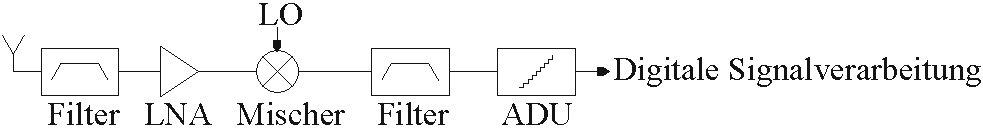
\includegraphics[width=14cm]{XX_DEMO_empfaenger} %Größe, Ort, am besten als vektorgraphik (pdf), Photos als jpg
\caption{Beschreibung (Quellen dahinter) \cite{BibDEMO1}\cite{BibDEMO2}}
\label{fig:textreferenz}
\end{figure}

Eine Quelle wird direkt hinter dem Satz vor dem Punkt angegeben mit \cite{BibDEMO1}, oder aber hinter einem kompletten Absatz. Auch Formeln (im Text) und Bilder (in der caption) müssen eine Quellenangabe enthalten.

Schöne Schaltpläne lassen sich auch direkt in Latex mi tikz/circuitikz malen, siehe \ref{tikz}.

\begin{figure}
	\centering
	\tikzsetnextfilename{XX_DEMO_tikz} %Dateiname, unter der die datei im ordner tikz-ext-out angelegt wird
	\tikzset{external/remake next} %uncomment to force remake figure
	\begin{tikzpicture}[scale=.8,transform shape]
	
	\draw  (0,0)coordinate[rground](start) to [vsourcesin,v<=$u_e$]++(0,3)to[R,l=$R_1$]++(4,0)coordinate[circ](knoten1)
			to [R,l=$R_3$]++(4,0) coordinate[circ](knoten2) --++(1,0) node[op amp,anchor=-](opv){};
			\draw (knoten1) to[C,l=$C_2$](knoten1|-start) coordinate[rground];
			\draw (knoten2) to[C,l=$C_1$]++(0,3) coordinate[circ](knoten3);
			\draw (knoten1) to[R,l=$R_2$]++(0,3)--(knoten3);
			\draw (opv.out)--++(1,0)|-(knoten3);
			\draw (opv.+)--++(-1,0)--++(0,-1)coordinate[rground];
			\draw (opv.out)++(1,0)to[short,*-o]++(1,0) coordinate(out);
			\draw  [->,shorten >=1ex,shorten <=1ex,thick] (out) -- (out|-start) node[left,midway] {\Large$u_a$};
			\draw (out|-start) coordinate[rground] coordinate[ocirc];
			
			\draw (knoten1) node[above left]{$\varphi_1$};
			\draw (knoten2) node[above left]{$\varphi_2$};
	\end{tikzpicture}
	\caption{Toller Schaltplan mit circuitikz (\url{https://github.com/lte-fau/circuitikz})}
	\label{tikz}
\end{figure}

\subsection{Formeln}

Auf Formeln kann mit \ref{eqn:tc} verwiesen werden. Konstanten und mathematische Funktionen (z.B. ln), sowie Einheiten sollten dabei nicht kursiv geschrieben werden. Zwischen einer Zahl und der Einheit ist ein halbes Leerzeichen mit 1,0\,\textmu V zu setzen. Das Komma ist bei der Zahl kein Punkt, die für Spannung steht das deutsche "`U"' und nicht "`V"'.

\begin{eqnarray}\label{eqn:tc}
X_{Strom}=\text{Konstante} \cdot 1,0\,\text{mV} \cdot \frac{1}{I} \cdot \frac{\partial I}{\partial T}
\end{eqnarray}

\subsection{Häufige Fehler}
Es sollten alle Dokumente im Format "utf8" gespeichert werden.

%Kommentare sind jederzeit mit einem %-Zeichen möglich
	
\chapter{Einleitung}
\label{sec:Einleitung}
\pagestyle{scrheadings}



noch unterzubringen:
wohin das Gehäuse?
\section{Motivation}

\section{Zieldefinition}

\section{Projektmanagement}

	%\input{Abschnitte/Grundlagen}
	%\input{Abschnitte/Stand_der_Technik}
	%\input{Abschnitte/Entwurf}
	%\input{Abschnitte/Aufbau}
	%\input{Abschnitte/Messung}
	%\input{Abschnitte/Zusammenfassung}
	%\input{Abschnitte/Fazit_und_Ausblick}
	%\input{Abschnitte/Literaturverzeichnis}
	\listoffigures
	\listoftables

	%\include{Abschnitte/Lebenslauf} 
	%\chapter{Anhang}
\label{sec:Anhang}
\pagestyle{scrheadings}
EINFÜGEN:
Layout Stefan Erhard
Bilder Altium
3D Modelle


\section{Seriennummern}
\label{app:Seriennummern}
Alle TDA5340 verfügen über eine eingebaute Seriennummer, welche ausgelesen werden kann. Die Seriennummern der verwendeten TDA5340 sind in der Tabelle aufgeführt.
\begin{table}[h]
\centering
\begin{tabular}{cc}
TDA & Seriennummer\\
\hline
TDA1 & 33020236\\
TDA2 & 11727080\\
TDA3& 11545236\\
TDA4& 11728870\\
TDA5& 11550773\\
TDA6& 33026263\\
\end{tabular}
\caption{Seriennummern der im Projekt verwendeten TDA5340 }
\label{default}
\end{table}%

\section{3D-Daten}
\subsection{Gehäuse}
\label{app:Gehäuse}
 
	
	\chapter*{Literatur}
	\printbibliography[heading=none]
\end{document}